\documentclass[12pt, a4paper]{article}

\usepackage[utf8]{inputenc}
\usepackage{mathtools}
\usepackage{amssymb}
\usepackage{ntheorem}
\usepackage[framemethod=TikZ]{mdframed}
\usepackage{amsmath}
\usepackage[hidelinks]{hyperref}
\usepackage{cleveref}
\usepackage[most]{tcolorbox}
\usepackage{fancyhdr}
\usepackage{lastpage}
\usepackage{geometry}
\usepackage{graphicx}
\usepackage{float} 
\usepackage{subfigure} 
\usepackage{arydshln}
\usepackage{float}
\usepackage{subfigure} 
\usepackage{multicol}
\usepackage{url}
\usepackage{setspace}
\usepackage{subfigure}
\usepackage[T1]{fontenc}
\usepackage{mathptmx}

\geometry{a4paper, left=2cm, right=2cm, bottom=2cm, top=2cm}

\definecolor{blue}{rgb}{0,0.45,1.14}
\definecolor{red}{rgb}{0.77,0.12,0.23}
\definecolor{grey}{rgb}{0.49,0.38,0.29}
\definecolor{green}{rgb}{0,0.42,0.24}
\definecolor{SpringGreen}{rgb}{0.95,0.97,0.95}
\definecolor{OliverGreen}{rgb}{0.09,0.34,0.09}
\definecolor{LeftGreen}{rgb}{0.13,0.54,0.13}
\definecolor{orange}{rgb}{2.07,0.69,0.32}

\newtcbtheorem[no counter]{example}{Example}{
  enhanced,
  sharp corners,
  attach boxed title to top left={
    yshifttext=-1mm
  },
  colback=white,
  colframe=blue!25,
  fonttitle=\bfseries,
  coltitle=black,
  boxed title style={
    sharp corners,
    size=small,
    colback=blue!25,
    colframe=blue!25,
  }
}{exm}

\newtcbtheorem[no counter]{theorem}{Theroem}{
  enhanced,
  sharp corners,
  attach boxed title to top left={
    yshifttext=-1mm
  },
  colback=white,
  colframe=grey!25,
  fonttitle=\bfseries,
  coltitle=black,
  boxed title style={
    sharp corners,
    size=small,
    colback=grey!25,
    colframe=grey!25,
  }
}{thm}

\newtcbtheorem[no counter]{proof}{Proof}{
  enhanced,
  sharp corners,
  attach boxed title to top left={
    yshifttext=-1mm
  },
  colback=white,
  colframe=orange!50,
  fonttitle=\bfseries,
  coltitle=black,
  boxed title style={
    sharp corners,
    size=small,
    colback=orange!50,
    colframe=orange!50,
  }
}{proof}

\newtcbtheorem{myclaim}{Definition}{ 
    coltitle=OliverGreen,
    colback=SpringGreen,
    colframe=LeftGreen,
    detach title,
    boxrule=0pt,
    leftrule=2pt,
    attach title to upper,
    sharp corners,
    left=1mm,
}{claim}

\rhead{\thepage}
\linespread{1.15}

\title{\textbf{IB Mathematics Analysis and Approaches HL}\\
Topic 2 Functions}
\author{Jiuru Lyu}
\date{\today}

\def\Z{{\mathbb{Z}}}
\def\R{{\mathbb{R}}}
\def\C{{\mathbb{C}}}
\def\Q{{\mathbb{Q}}}
\def\E{{\mathbb{E}}}
\def\d{{\mathrm{d}}}

\begin{document}

\maketitle
\tableofcontents

\newpage

\section{Foundations of Functions}
\begin{enumerate}
    \item Relations and functions: 
    \begin{myclaim}{ }{}
        A \textbf{\color{red}{relation}} $R$ is a set of ordered pairs $(x,y)$ such that $x\in A,\ y\in B$, and sets $A,\ B$ are not empty. 
    \end{myclaim}
    \begin{myclaim}{ }{}
        A \textbf{\color{red}{function}} $f$ is a relation in which every $x$-value has a unique $y$-value. 
    \end{myclaim}
    \item Domain and Range: 
    \begin{myclaim}{ }{}
        \textbf{\color{red}{Domain}} is the set of $x$-values. 
    \end{myclaim}
    \begin{myclaim}{ }{}
        \textbf{\color{red}{Range}} is the set of $y$-values. 
    \end{myclaim}
    \begin{itemize}
        \item Domain and Range should be in inverval notation. 
        \begin{enumerate}
            \item Using invervals to express the inequalities
            \begin{example}{2.1.2}{}
                $$\left[\right.3,4\left[\right. \text{ means }3\leq x<4$$
            \end{example}
            \item If the interval will be joint, we use ${\color{red}{\cup}}$ to join the inverval. 
            \begin{example}{2.1.2}{}
                $$3<x<4\text{ or }x\geq 5\ \Rightarrow\ \left.\right]3,4\left.\right]\cup\left[5,+\infty\right.\left[\right.$$
            \end{example}
            \begin{example}{2.1.3}{}
                \textbf{Find the interval notation for the domain of $\displaystyle f(x)=\frac{1}{x}$.}\\
                \noindent\rule[0.1pt]{\textwidth}{1pt}
                $$x\in\left.\right]-\infty,0\left[\right.\cup\left.\right]0,+\infty\left[\right.\text{ OR } x\in\R\setminus 0$$
                {\color{green}{Note: $\setminus$ means "exclude."}}
            \end{example}
        \end{enumerate}
        \item Since the $y$-values (outputs) depend on the $x$-values (inputs), $y$ is the \textbf{\color{red}{dependent variable}}, and $x$ is the \textbf{\color{red}{independent variable}}.
        \item The independent vairbale $x$ is also called the \textbf{\color{red}{argument}} of the function. 
    \end{itemize}
    \item Vertical Line test: 
    \begin{itemize}
        \item To test whether a relation is a function. 
        \item Since every $x$ has one and only one value of $y$, there should be only one intersects. 
    \end{itemize}
    \item Inverse of a function: 
    \begin{myclaim}{ }{}
        $f^{-1}(x)$ is the \textbf{\color{red}{inverse function}} of $f(x)$.
        \begin{figure}[H]
            \centering
            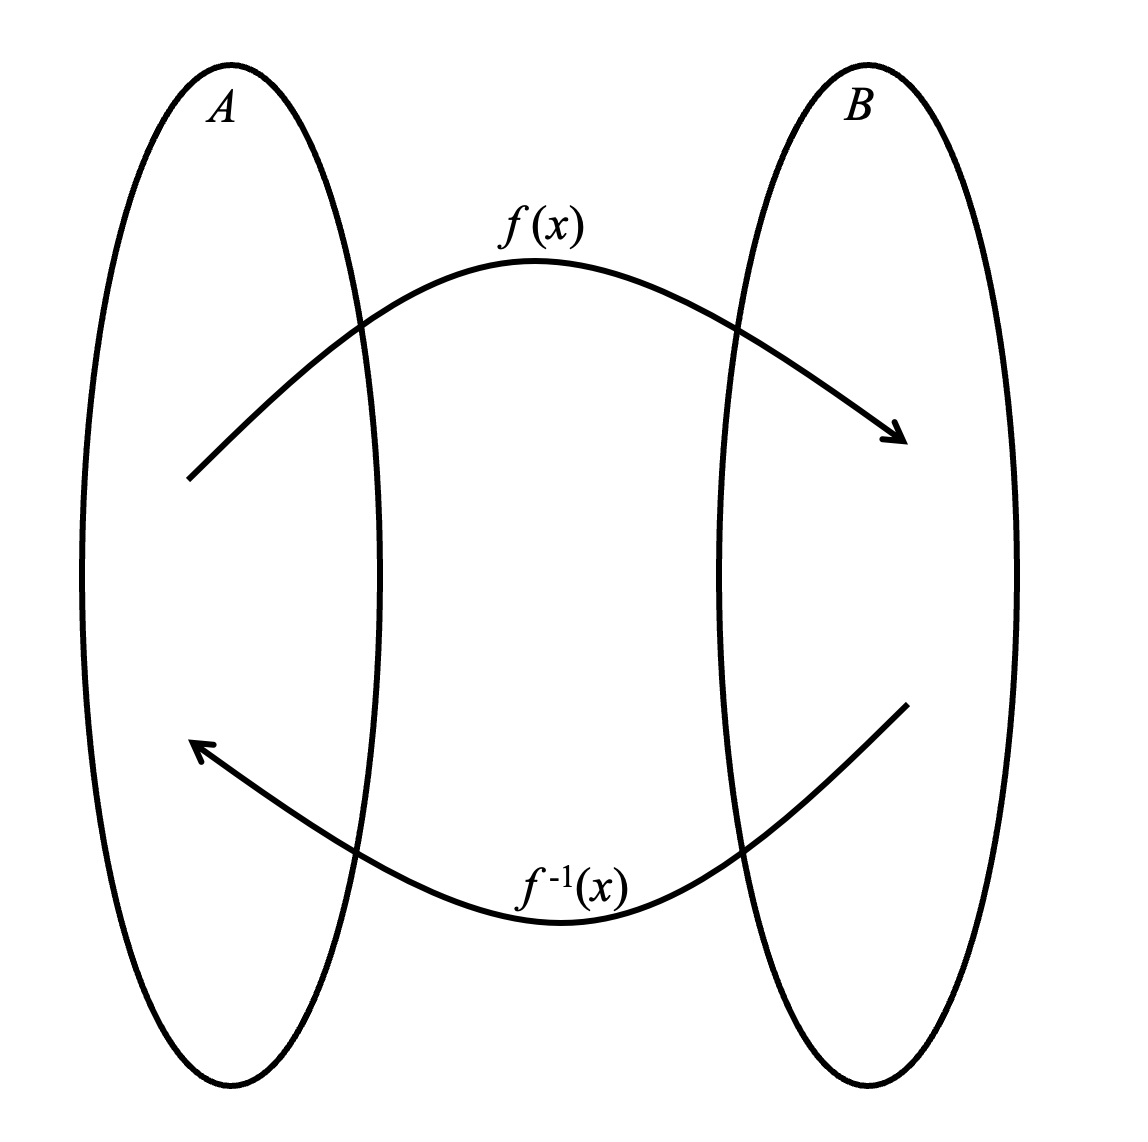
\includegraphics[width=0.5\textwidth]{Fig.2.1.jpg}
          \end{figure}
    \end{myclaim}
    \begin{example}{2.1.3}{}
        $f(1)=3\ \Rightarrow\ f^{-1}(3)=1;\ f(x)=x+5\ \Rightarrow\ f^{-1}(x)=x-5$
    \end{example}
    \begin{itemize}
        \item In inverse function, the input becomes the output, the output becomes the input. 
        \item In inverse function, the domain becomes the range, the range becomes the domain. 
        \begin{example}{2.1.4}{}
            \begin{enumerate}
                \item \textbf{Find the inverse function of $\displaystyle y=\frac{x+2}{3}$.}\\
                \noindent\rule[0.1pt]{0.9\textwidth}{1pt}
                $$\begin{aligned}
                    3y=x+2&\Rightarrow x=3y-2\\
                    f^{-1}(x)&=3x-2
                \end{aligned}$$
                \item \textbf{Find the inverse function of $f(x)=\displaystyle \frac{x}{x+1}$.}\\
                \noindent\rule[0.1pt]{0.9\textwidth}{1pt}
                $$\begin{aligned}
                    y=\frac{x}{x+1}\Rightarrow xy+y=x&\Rightarrow xy+x=y\\
                    \therefore y(x-1)=-x&\Rightarrow y=-\frac{x}{x-1}
                \end{aligned}$$
                \item \textbf{Find the inverse of $\{.(4,2),(0,2),(-2,2)\}$}\\
                \noindent\rule[0.1pt]{0.9\textwidth}{1pt}
                $$\text{Inverse: }\{(2,4),(2,0),(2,-2)\}$$
            \end{enumerate}
        \end{example}
        \item By restricting the domain, we can find $f^{-1}(x)$ of $f(x)$, if the direct inverse of $f(x)$ is not a function.
        \begin{example}{2.1.5}{}
            \begin{figure}[H]
                \centering
                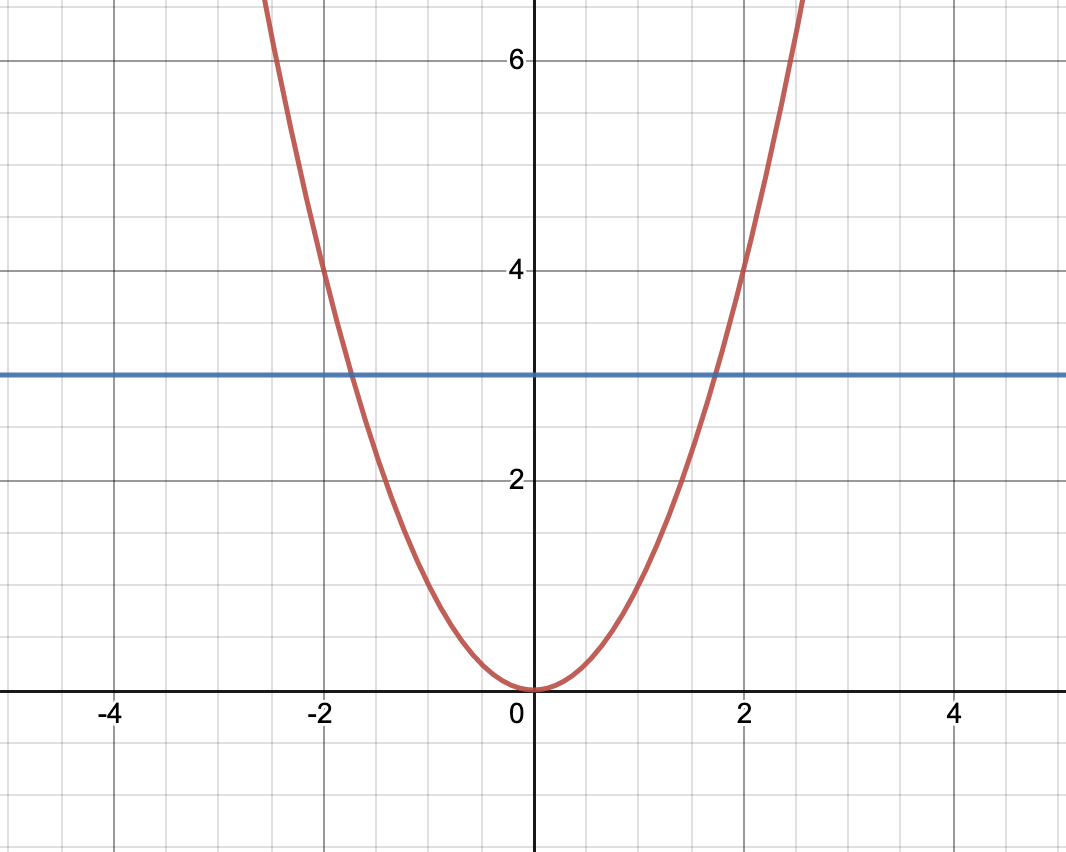
\includegraphics[width=0.5\textwidth]{Fig.2.2.jpg}
              \end{figure}
              {\color{red}{Horizontal line test}}: The largest domain we can find $f^{-1}(x)$ is $x\leq 0$ or $x>0$.
        \end{example} 
    \end{itemize}
    \item Composite Functions: 
    \begin{myclaim}{ }{}
        We use {\color{red}$(g\circ h)(x)$} or {\color{red}{$g(h(x))$}} to represent composite functions. 
        \begin{figure}[H]
            \centering
            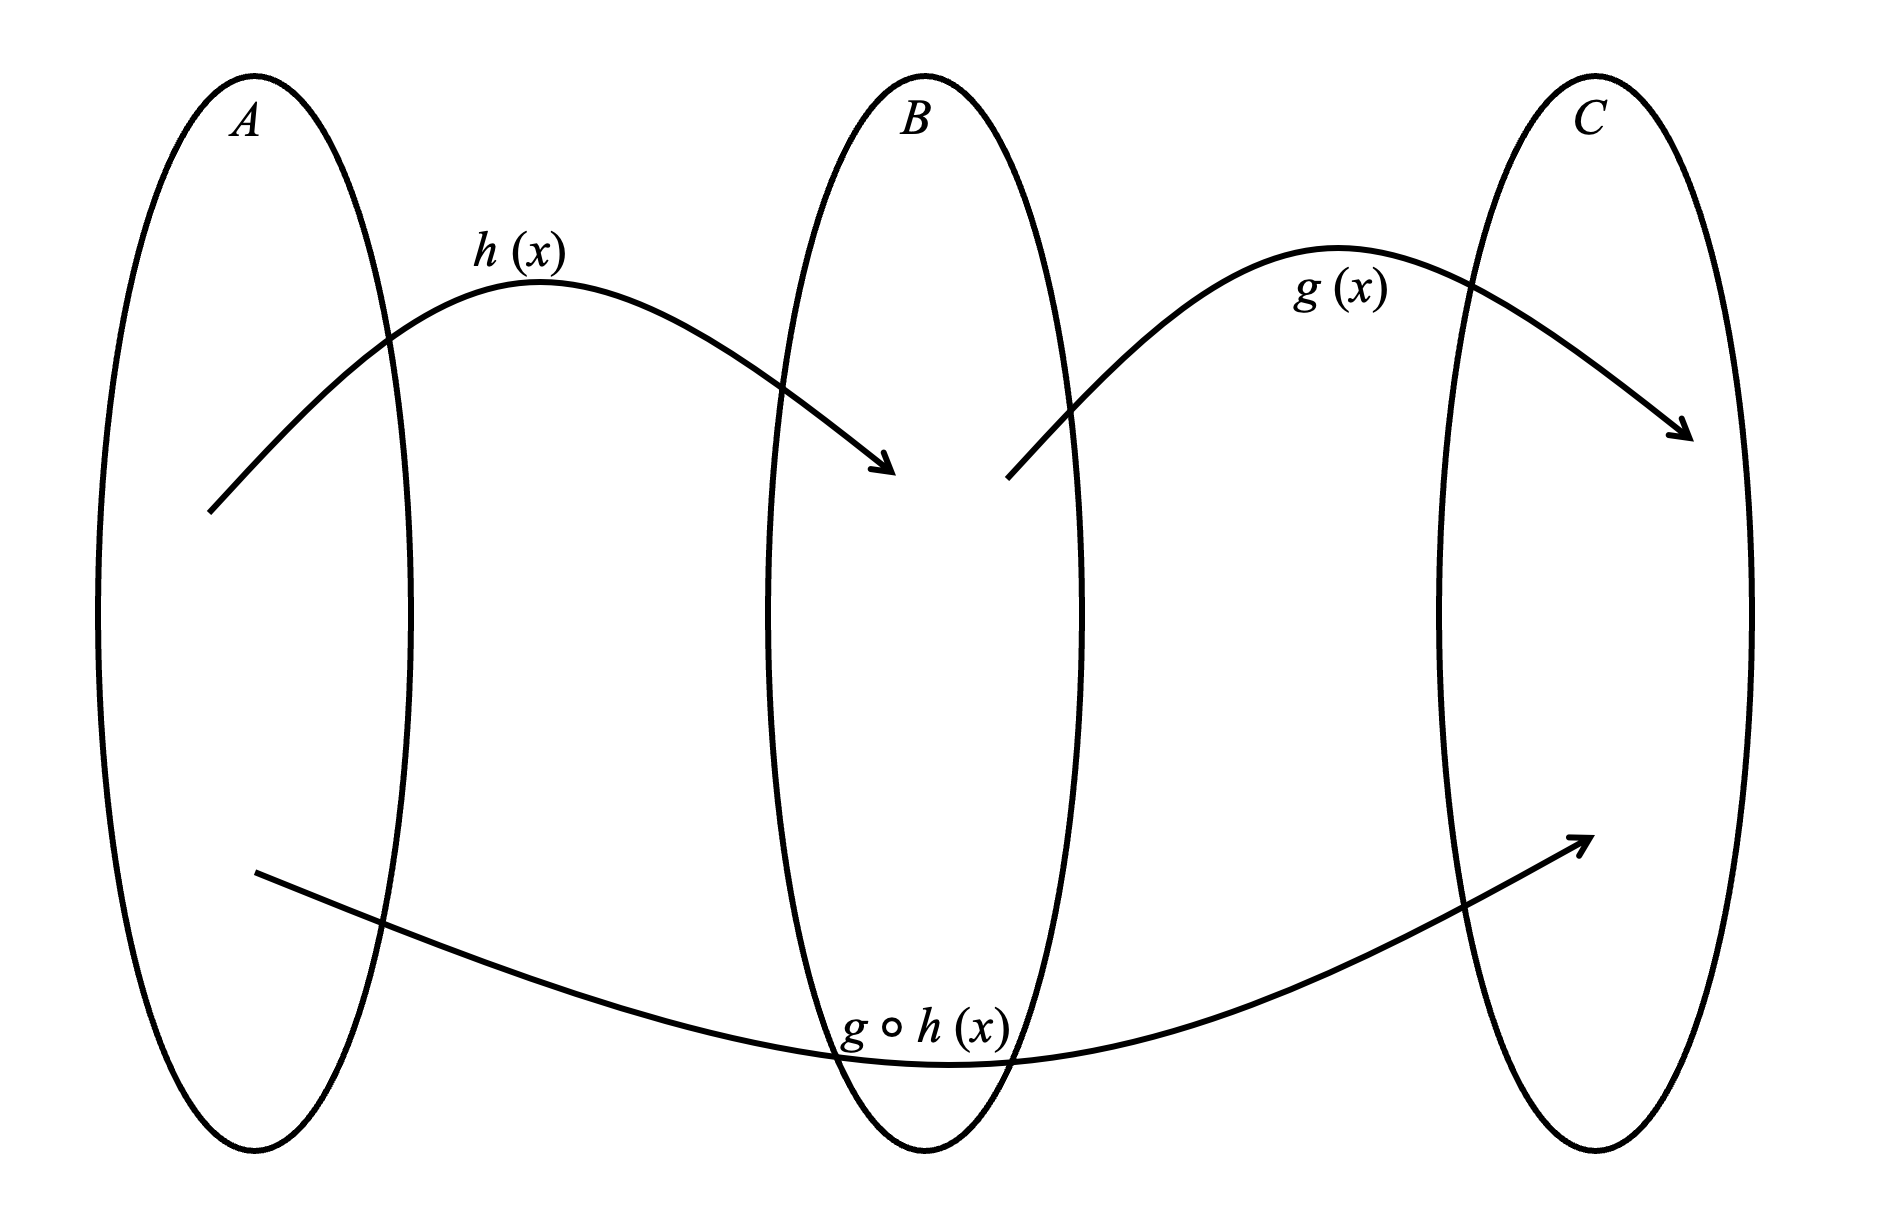
\includegraphics[width=0.7\textwidth]{Fig.2.3.jpg}
          \end{figure}
    \end{myclaim}
    \begin{example}{2.1.6}{}
        \textbf{Given $f:x\mapsto  3x-6,\ g:x\mapsto\displaystyle\frac{1}{3}x+2$. Find $(f\circ g)(x)$ and $(g\circ f)(x)$.}\\
        \noindent\rule[0.1pt]{\textwidth}{1pt}
        $$(f\circ g)(x)=f\left(g(x)\right)=3(\frac{1}{3}x+2)-6=x.$$
        $$(g\circ f)(x)=g\left(f(x)\right)=\frac{1}{3}(3x-6)+2=x.$$
    \end{example}
    When $f$ and $g$ are inverse functions: $${\color{red}{(f\circ g)(x)(x)=x=(g\circ f)(x)}}.$$
    \item $f(x)$ and $f^{-1}(x)$ are symmetrical to $y=x$ since $D_f=R_{f^{-1}}$, $R_f=D_{f^{-1}}$. That is, {\color{red}{if $f(x)$ passes through $(a,b)$, $f^{-1}(x)$ passes through $(b,a)$}}.
\end{enumerate}

\section{Quadratic Functions}
\begin{enumerate}
    \item The Standard Form: 
    $$\color{red}{y=ax^2+bx+c},$$
    where $a$ is the coefficient of $x^2$, $b$ is the coefficient of x, and $c$ is the constant or $y$-intercept. $a,b,c\neq 0$. 
    \begin{itemize}
        \item Zeros of the function ($x$-intercepts): 
        $$\color{red}{x=\frac{-b\pm\sqrt{b^2-4ac}}{2a}},$$
        where $\Delta=b^2-4ac$ is the discriminant of the function. 
        \item Euqation of the line of symmetry \& $x$-coordinate of the vertex
        $$x=-\frac{b}{2a}.$$
        \item Vieta's Formula: 
        \begin{theorem}{2.2.1: The Vieta's Theorem}{}
            Assume $x_1,\ x_2$ are two roots for equation $ax^2+bx+c=0\ (a\neq 0)$, then
            $$\color{red}x_1+x_2=-\frac{b}{a};$$
            $$\color{red}x_1\cdot x_2=\frac{c}{a}.$$
        \end{theorem}
        \item When $a>0,$ the parabola opens upwards. \\
        When $a<0$, the parabola opens downwards.
    \end{itemize}
    \item Completion of square: 
    $${\color{red}{x^2+px+\left(\frac{p}{2}\right)^2-\left(\frac{p}{2}\right)^2=\left(x+\frac{p}{2}\right)^2-\left(\frac{p}{2}\right)^2}}.$$
    \item The Vertex Form: 
    $${\color{red}{y=a(x-h)^2+k,\text{ where }(h,k)\text{ is the vertex}}}.$$
    \begin{example}{2.2.1}{}
        \textbf{Given that $f(x)=ax^2+bx+c,$ find the axis of symmetry and vertex.}\\
        \noindent\rule[0.1pt]{\textwidth}{1pt}
        $$\begin{aligned}
            f(x)&=a\left(x^2+\frac{b}{a}x\right)+c\\
            &=a\left[x^2+\frac{b}{a}x+\left(\frac{b}{2a}\right)^2\right]+c-\frac{b^2}{4a}\\
            &=a\left(x+\frac{b}{2a}\right)^2+\frac{4ac-b^2}{4a}.
        \end{aligned}$$
        $$\begin{aligned}
            \therefore \text{ axis of symmetry: }&x=-\frac{b}{2a}\\
            \text{vertex: }&\left(-\frac{b}{2a},\frac{4ac-b^2}{4a}\right).
        \end{aligned}$$
    \end{example}
\end{enumerate}

\section{Higher Order Polynomial Functions}
\begin{enumerate}
    \item Factor Theorem: 
    \begin{theorem}{2.3.1: The Factor Theorem}{}
        If $(x-a)$ is a factor of a polynomial $P(x)$, then $x=a$ must be a root for $P(x)\ \Rightarrow {\color{red}{P(a)=0}}$.
        \begin{proof}{2.3.1}{}
            Assume the quotient when $P(x)$ is divided by $(x-a)$ is $Q(x)$, then $P(x)=Q(x)\cdot(x-a)$. Then, $P(a)=Q(a)\cdot(a-a)=0$.
        \end{proof}
    \end{theorem}
    \item Long division: solving polynomial equation. 
    \begin{example}{2.3.1}{}
        \textbf{For a cubic function, $P(x)=2x^3+bx^2+cx+d,\ P(1)=P(2)=P(3)=2.$ What is $P(0)$?}\\
        \noindent\rule[0.1pt]{\textwidth}{1pt}
        Since $P(1)=P(2)=P(3)=2, Q(1)=Q(2)=Q(3)=0,\text{ where }Q(x)=P(x)-2.$\\
        Thus, $Q(x)=2(x-1)(x-2)(x-3).$
        $$\therefore P(x)=Q(2)+2=2(x-1)(x-2)(x-3)+2.$$
        $$\therefore P(0)=2(-1)(-2)(-3)+2=-10.$$
    \end{example}
    \item Remainder Theorem: 
    \begin{theorem}{2.3.2: The Remainder Theorem}{}
        When a polynomial $P(x)$ is divided by $(ax-b)$, the remainder $R$ of this division must be $${\color{red}{P\left(\frac{b}{a}\right)}}.$$
        \begin{proof}{2.3.2}{}
            Assume the quotient is $Q(x)$, and the reminder is $R$: 
            $$P(x)=(ax-b)Q(x)+R.$$
            $$P\left(\frac{b}{a}\right)=0\cdot Q(X)+R=R.$$
        \end{proof}
    \end{theorem}
    \item Roots of Cubic Functions: 
    \begin{theorem}{2.3.3}{}
        For a cubic function $f(x)=ax^3+bx^2+cx+d$, given the roots of it are $\alpha,\ \beta$, and $\gamma$. Then, 
        $${\color{red}{\begin{cases}
            \alpha+\beta+\gamma=-\displaystyle\frac{b}{a}\ \Rightarrow\ \sum\alpha=-\frac{b}{a}\\
            \displaystyle\alpha\beta+\alpha\gamma+\beta\gamma=\frac{c}{a}\ \Rightarrow\ \sum\alpha\beta=\frac{c}{a}\\
            \displaystyle\alpha\beta\gamma=-\frac{d}{a}\ \Rightarrow\ \sum\alpha\beta\gamma=-\frac{d}{a}
        \end{cases}}}$$
        \begin{proof}{2.3.3}{}
            Since $\alpha,\ \beta,\ \gamma$ are roots of $f(x)$, 
            $$f(x)=a(x-\alpha)(x-\beta)(x-\gamma).$$
            $$\text{So } a(x-\alpha)(x-\beta)(x-\gamma)=ax^3+bx^2+cx+d,$$
            $$\text{i.e., }ax^3-a(\alpha+\beta+\gamma)x^2+a(\alpha\beta+\alpha\gamma+\beta\gamma)x-a\alpha\beta\gamma=ax^3+bx^2+cx+d.$$
            $$\Rightarrow\ \alpha+\beta+\gamma=-\frac{b}{a}, \alpha\beta+\alpha\gamma+\beta\gamma=\frac{c}{a}, \alpha\beta\gamma=-\frac{d}{a}.$$
        \end{proof}
        \begin{theorem}{2.3.4: An extention to Theorem 2.3.3}{}
            $$\sum\alpha=-\frac{b}{a},\ \sum\alpha\beta=\frac{c}{a},\ \sum\alpha\beta\gamma=-\frac{d}{a},\ \sum\alpha\beta\gamma\delta=\frac{e}{a}.$$
        \end{theorem}
    \end{theorem}
\end{enumerate}

\section{Rational Functions}
\begin{enumerate}
    \item Reciprocal Functions: $f(x)=\displaystyle \frac{1}{x}$.
    \begin{itemize}
        \item Domain: $x\in\R,\ x\neq 0$
        \item As $x$ increases, $\displaystyle\frac{1}{x}$ decreases $\Rightarrow x\rightarrow\infty, \displaystyle\frac{1}{x}\rightarrow 0$.
        \item Range: $y\in\R,\ y\neq 0$
        \item \textbf{\color{red}{Asymptotes}}: $x=0$, $y=0$. 
        \item Axis of symmetry: $y=x$, $y=-x$.
        \item \textbf{\color{red}{Self-inversing function}}: have axis of symmetry $y=x$. $$f(x)=f^{-1}(x).$$
    \end{itemize}
    \item $\displaystyle y=\frac{a}{bx+c}$
    \begin{itemize}
        \item Vertical asymptotes (V.A.): $bx+c=0$
        \item Horizontal asymptotes (H.A.): $y=0$
        \begin{example}{2.4.1}{}
            \textbf{Draw the diagram of $\displaystyle y=\frac{5}{3x-1}$.}\\
            \noindent\rule[0.1pt]{\textwidth}{1pt}
            $x$-intercept: $0=\frac{5}{3x-1}\Rightarrow$ no solution, no intercept.\\
            H.A.: $y=0$\\
            $y$-intercept: $y=-5$\\
            V.A.: $3x-1=0,\ x=\displaystyle\frac{1}{3}$
            \begin{figure}[H]
                \centering
                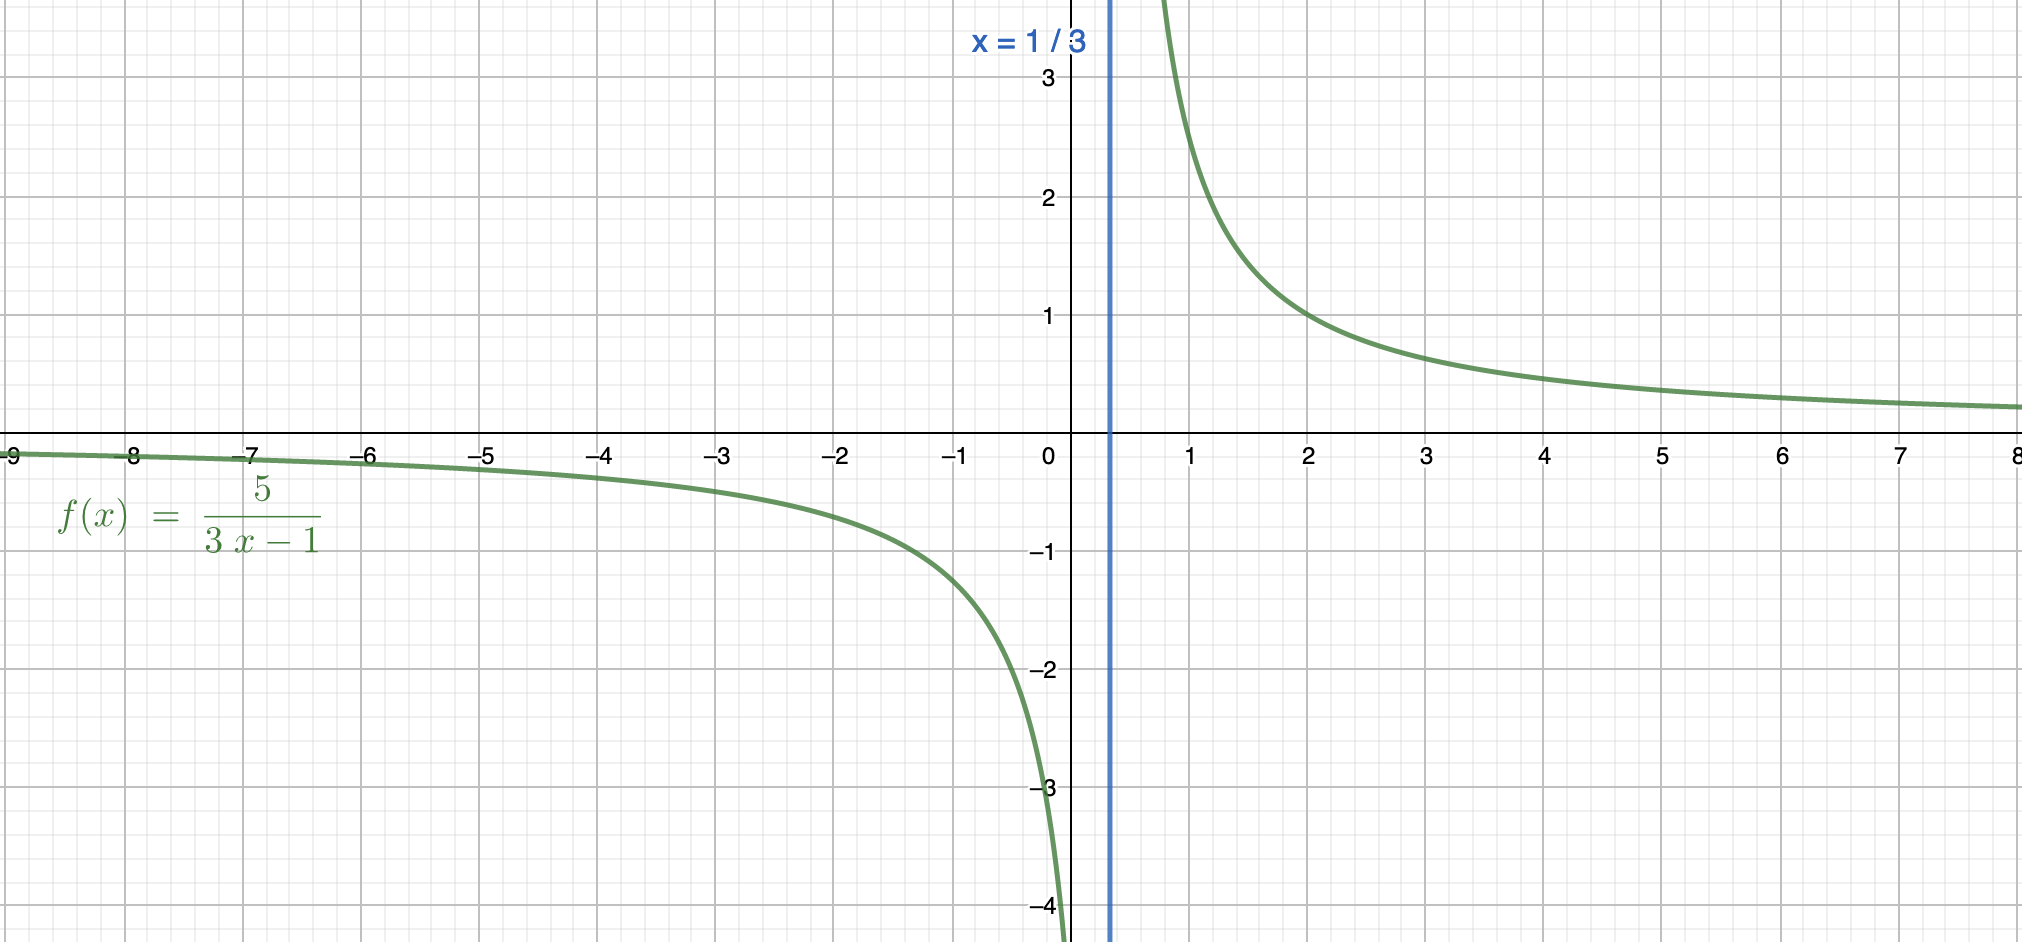
\includegraphics[width=0.8\textwidth]{Fig.2.4.jpg}
            \end{figure}
        \end{example}
    \end{itemize}
    \item $\displaystyle y=\frac{ax+b}{cx+d}$
    \begin{itemize}
        \item V.A.: $cx+d=0$
        \item H.A.: $y=\displaystyle\frac{a}{c}$
    \end{itemize}
    \item $\displaystyle y=\frac{ax+b}{cx^2+dx+e}$
    \begin{itemize}
        \item V.A.: $cx^2+dx+e=0$
        \item H.A.: As $\displaystyle x\to\pm\infty,\ \frac{ax}{cx^2}\to 0$, $y=0$
        \item Intercepts: $\displaystyle\left(0,\frac{e}{c}\right),\ \left(-\frac{e}{d},0\right)$
        \begin{example}{2.4.2}{}
            \textbf{Draw the diagram of $\displaystyle y=\frac{2x-6}{x^2-3x-4}$.}\\
            \noindent\rule[0.1pt]{\textwidth}{1pt}
            Intercept: $\displaystyle\left(0,\frac{3}{2}\right),\ \left(3,0\right)$\\
            H.A.: $y=0$\\
            V.A.: $x=-1,\ x=4$
            \begin{figure}[H]
                \centering
                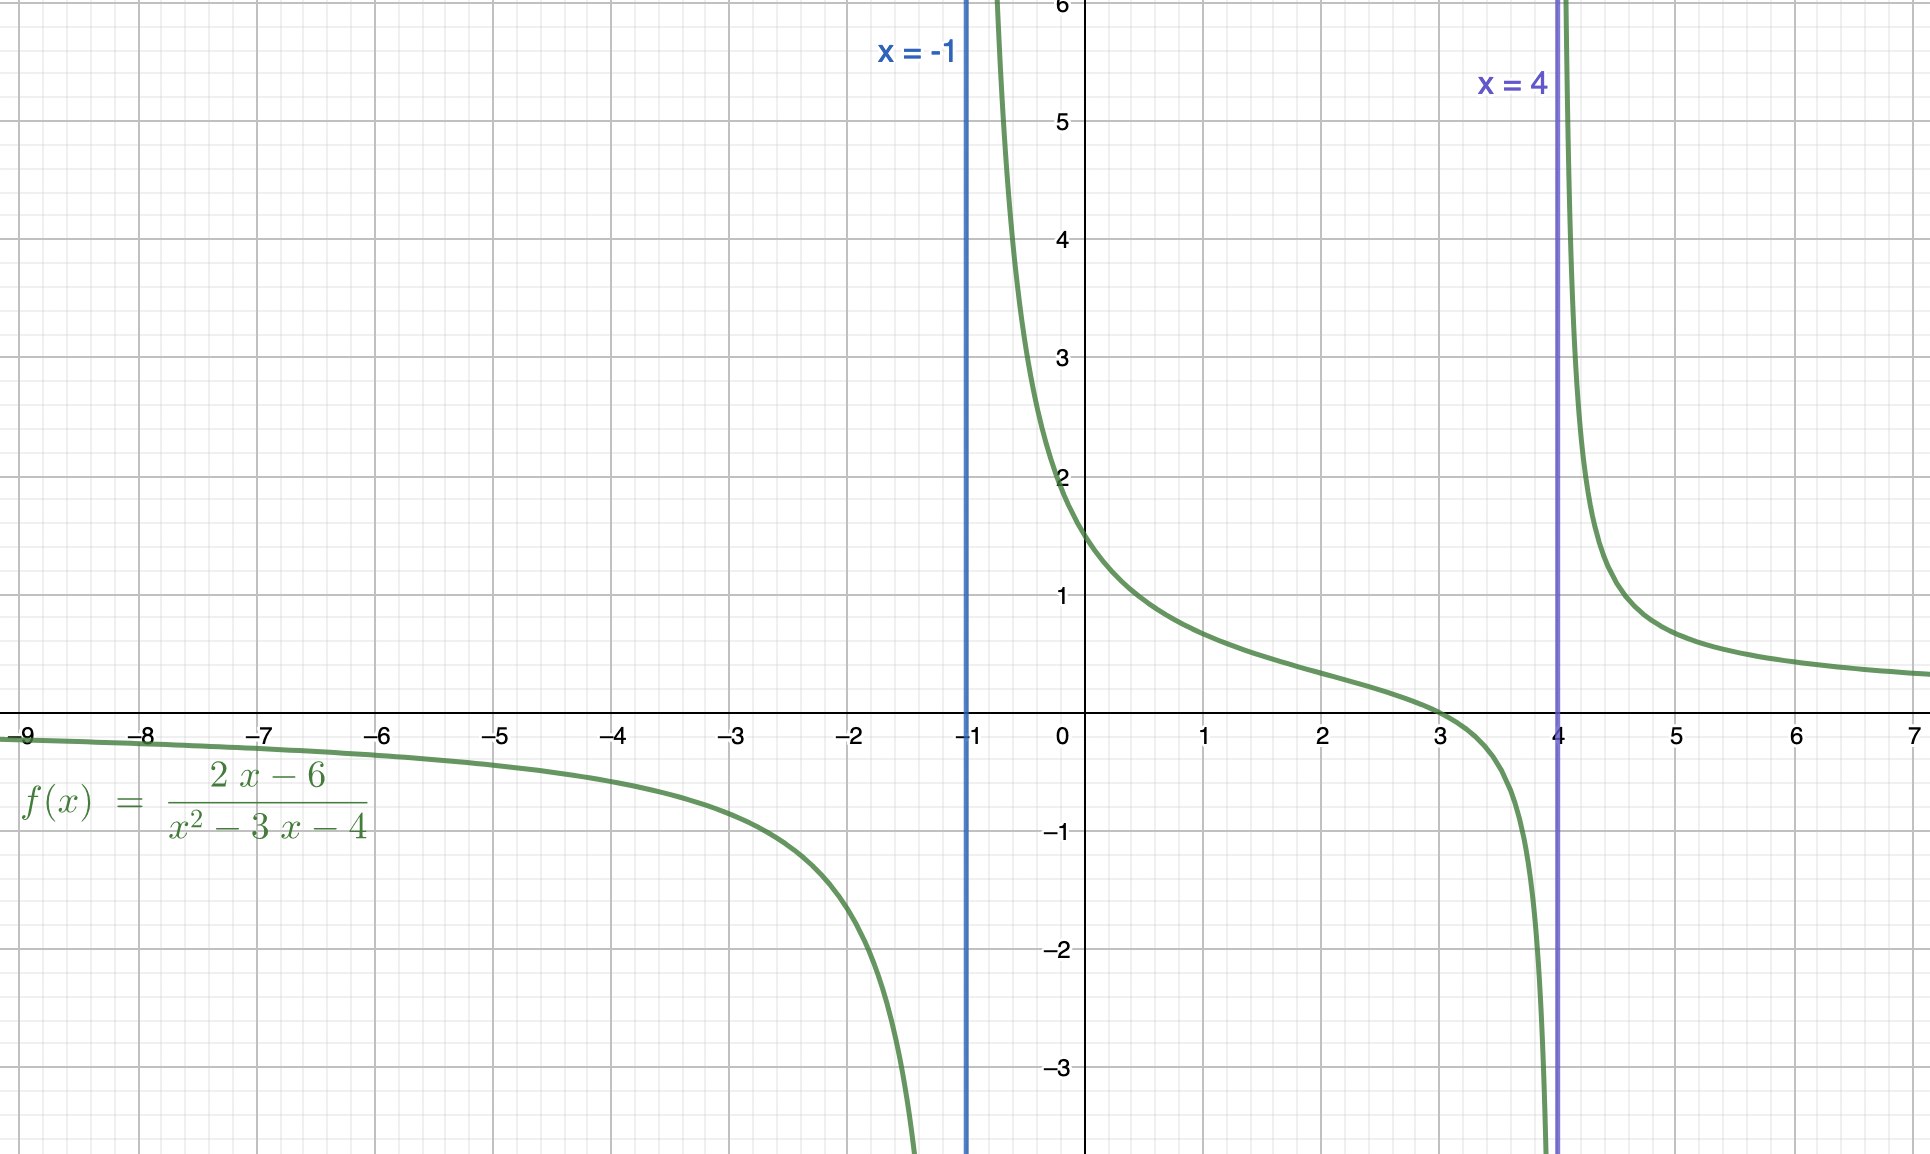
\includegraphics[width=0.8\textwidth]{Fig.2.5.jpg}
            \end{figure}
        \end{example}
        \begin{example}{2.4.3}{}
            \textbf{Draw the diagram of $\displaystyle y=\frac{3x+6}{x^2+2x+1}$.}\\
            \noindent\rule[0.1pt]{\textwidth}{1pt}
            Intercept: $\displaystyle\left(0,6\right),\ \left(-2,0\right)$\\
            H.A.: $y=0$\\
            V.A.: $x=-1$
            \begin{figure}[H]
                \centering
                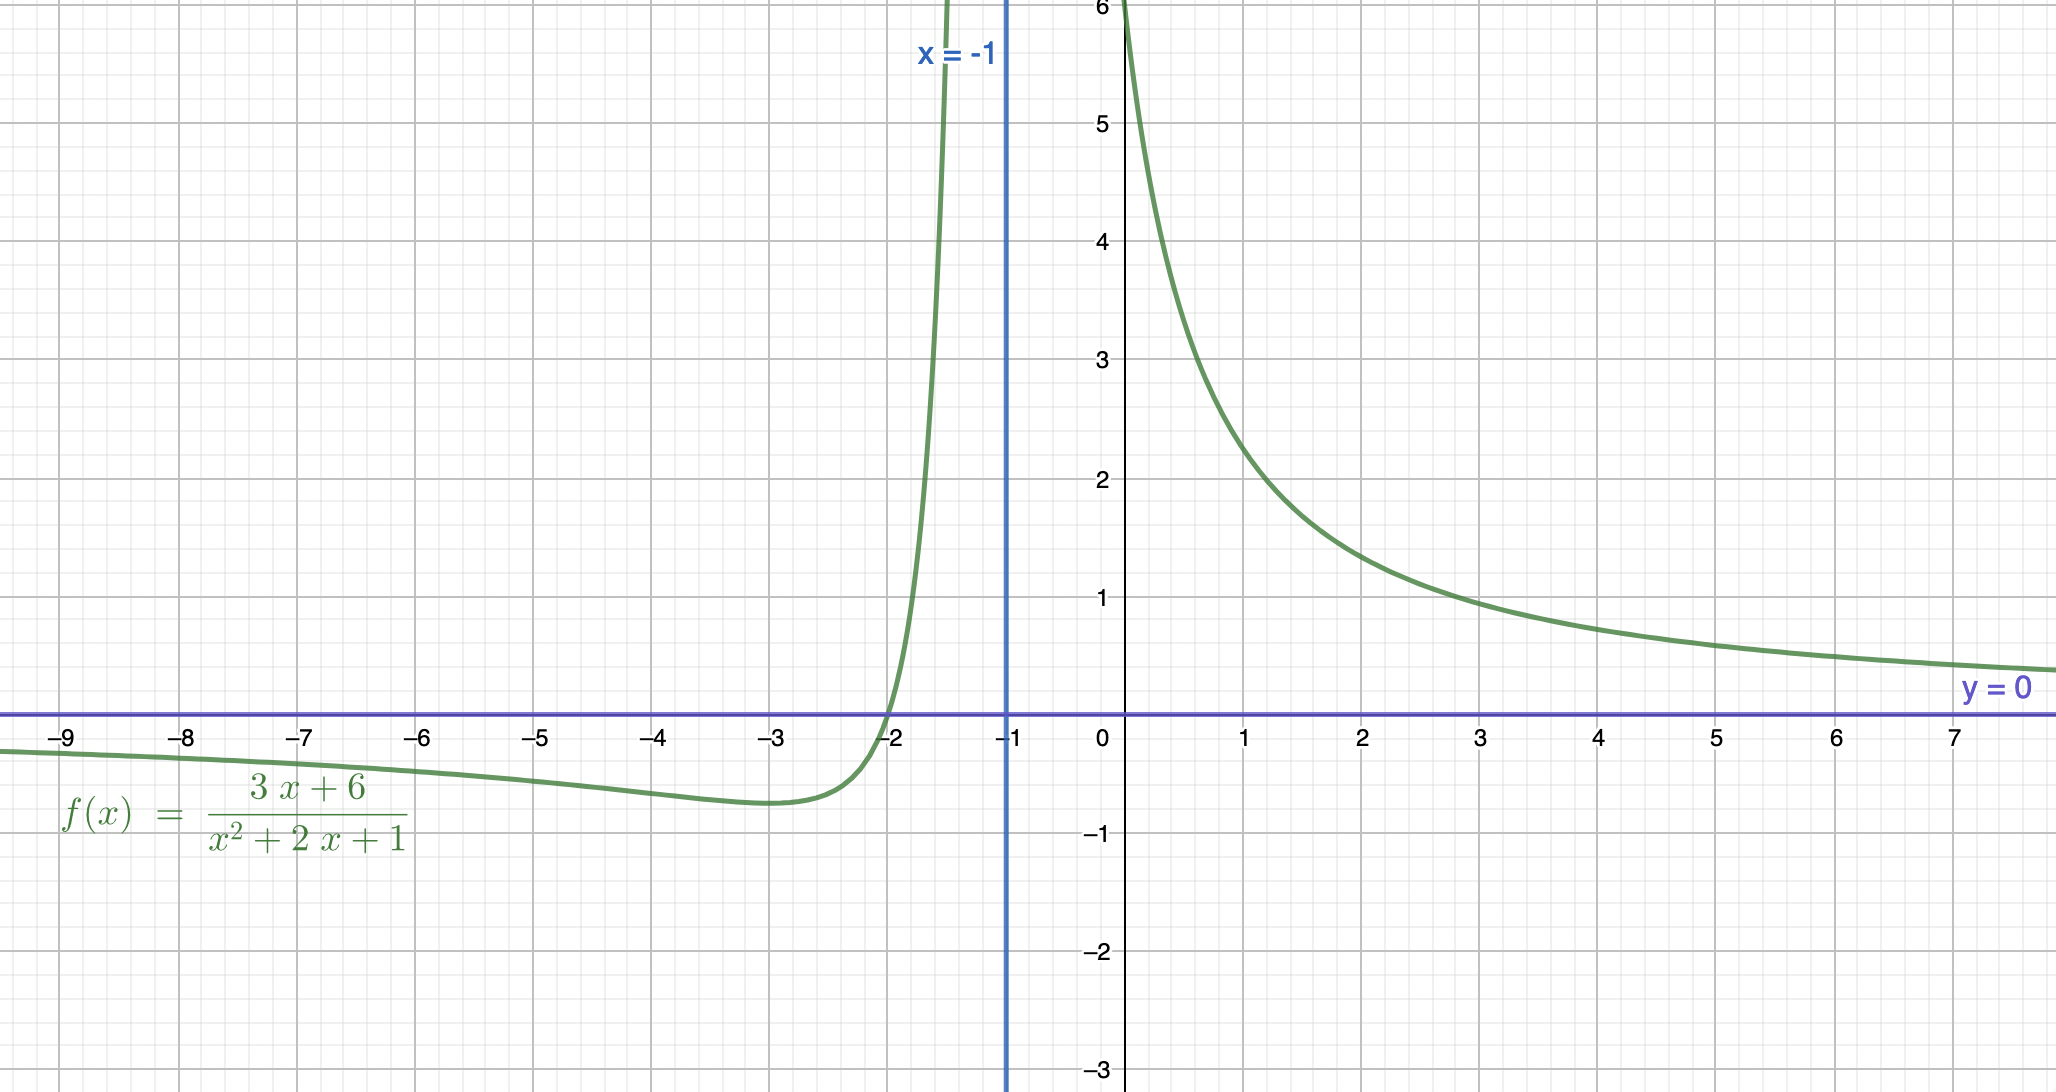
\includegraphics[width=0.8\textwidth]{Fig.2.6.jpg}
            \end{figure}
        \end{example}
        \begin{example}{2.4.4}{}
            \textbf{Draw the diagram of $\displaystyle y=\frac{x-6}{x^2+2x+3}$.}\\
            \noindent\rule[0.1pt]{\textwidth}{1pt}
            Intercept: $\displaystyle\left(6,0\right),\ \left(0,-2\right)$\\
            When $x\to\infty,\ f(x)$ is positive. When $x\to -\infty,\ f(x)$ is negative. 
            \begin{figure}[H]
                \centering
                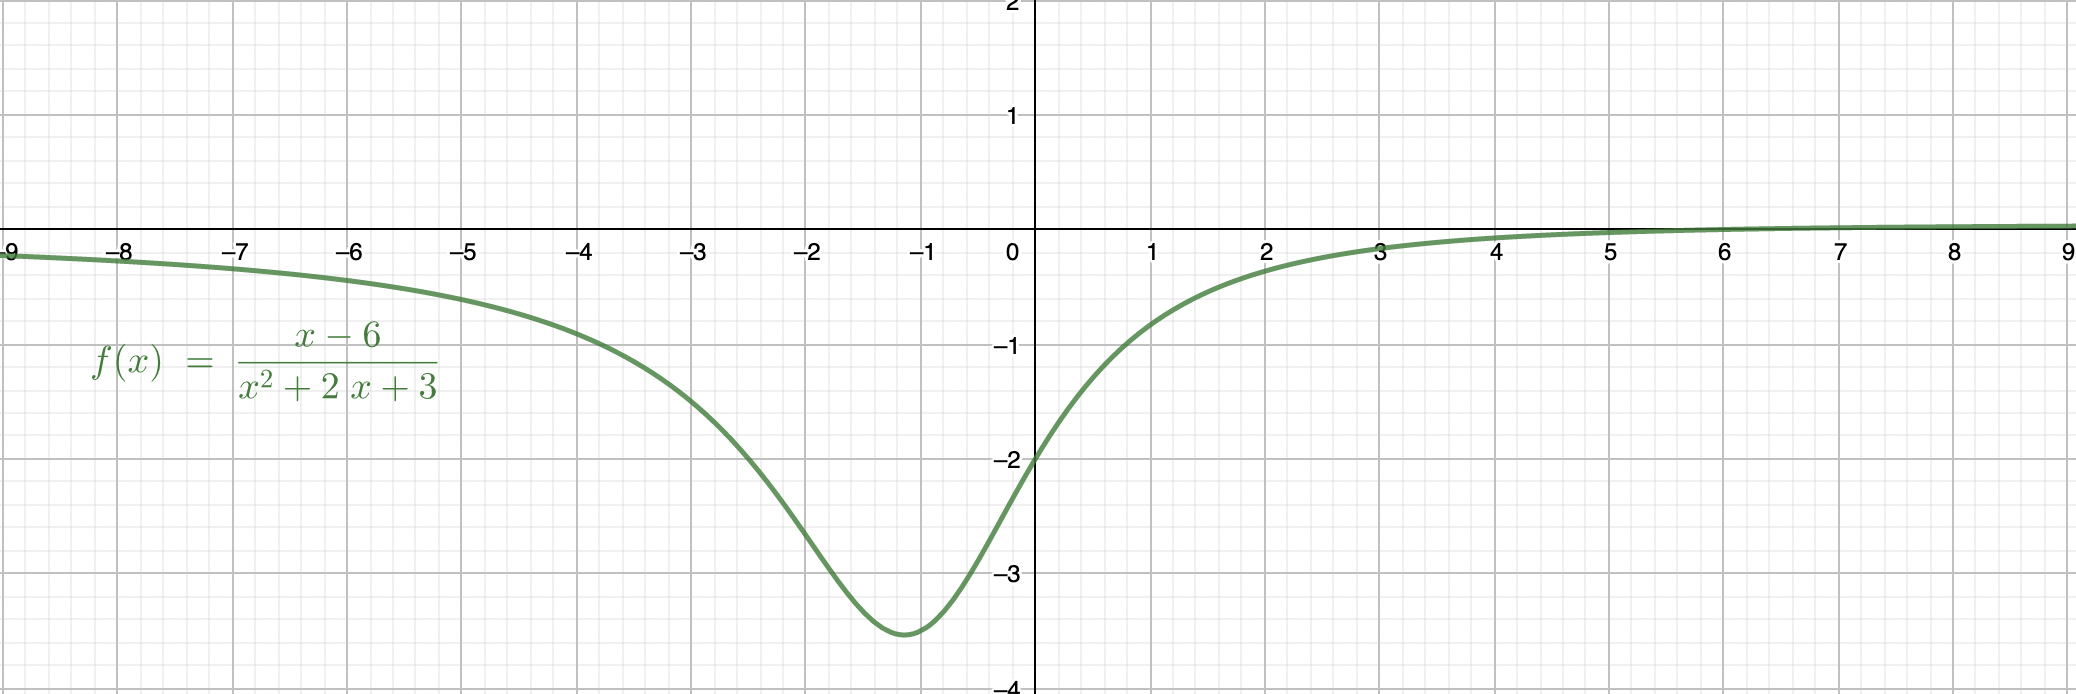
\includegraphics[width=0.8\textwidth]{Fig.2.7.jpg}
            \end{figure}
        \end{example}
    \end{itemize}
    \item $\displaystyle y=\frac{ax^2+bx+c}{dx+e}$
    \begin{itemize}
        \item V.A.: $dx+e=0$
        \item \textbf{\color{red}{Oblique Asymptote}}: Quotient of $(ax^2+bx+c)$ dividied by $(dx+e)$.
        \item Intercepts: $\displaystyle \left(0, \frac{c}{e}\right),\ ax^2+bx+c=0$
        \begin{example}{2.4.5}{}
            \textbf{Draw the diagram of $\displaystyle y=\frac{x^2+3x+2}{x-2}$.}\\
            \noindent\rule[0.1pt]{\textwidth}{1pt}
            Intercept: $\displaystyle\left(0,-1\right),\ \left(-1,0\right),\ \left(-2,0\right)$\\
            V.A.: $x=2$\\
            O.A.: $y=x+5$ (Use long division)
            \begin{figure}[H]
                \centering
                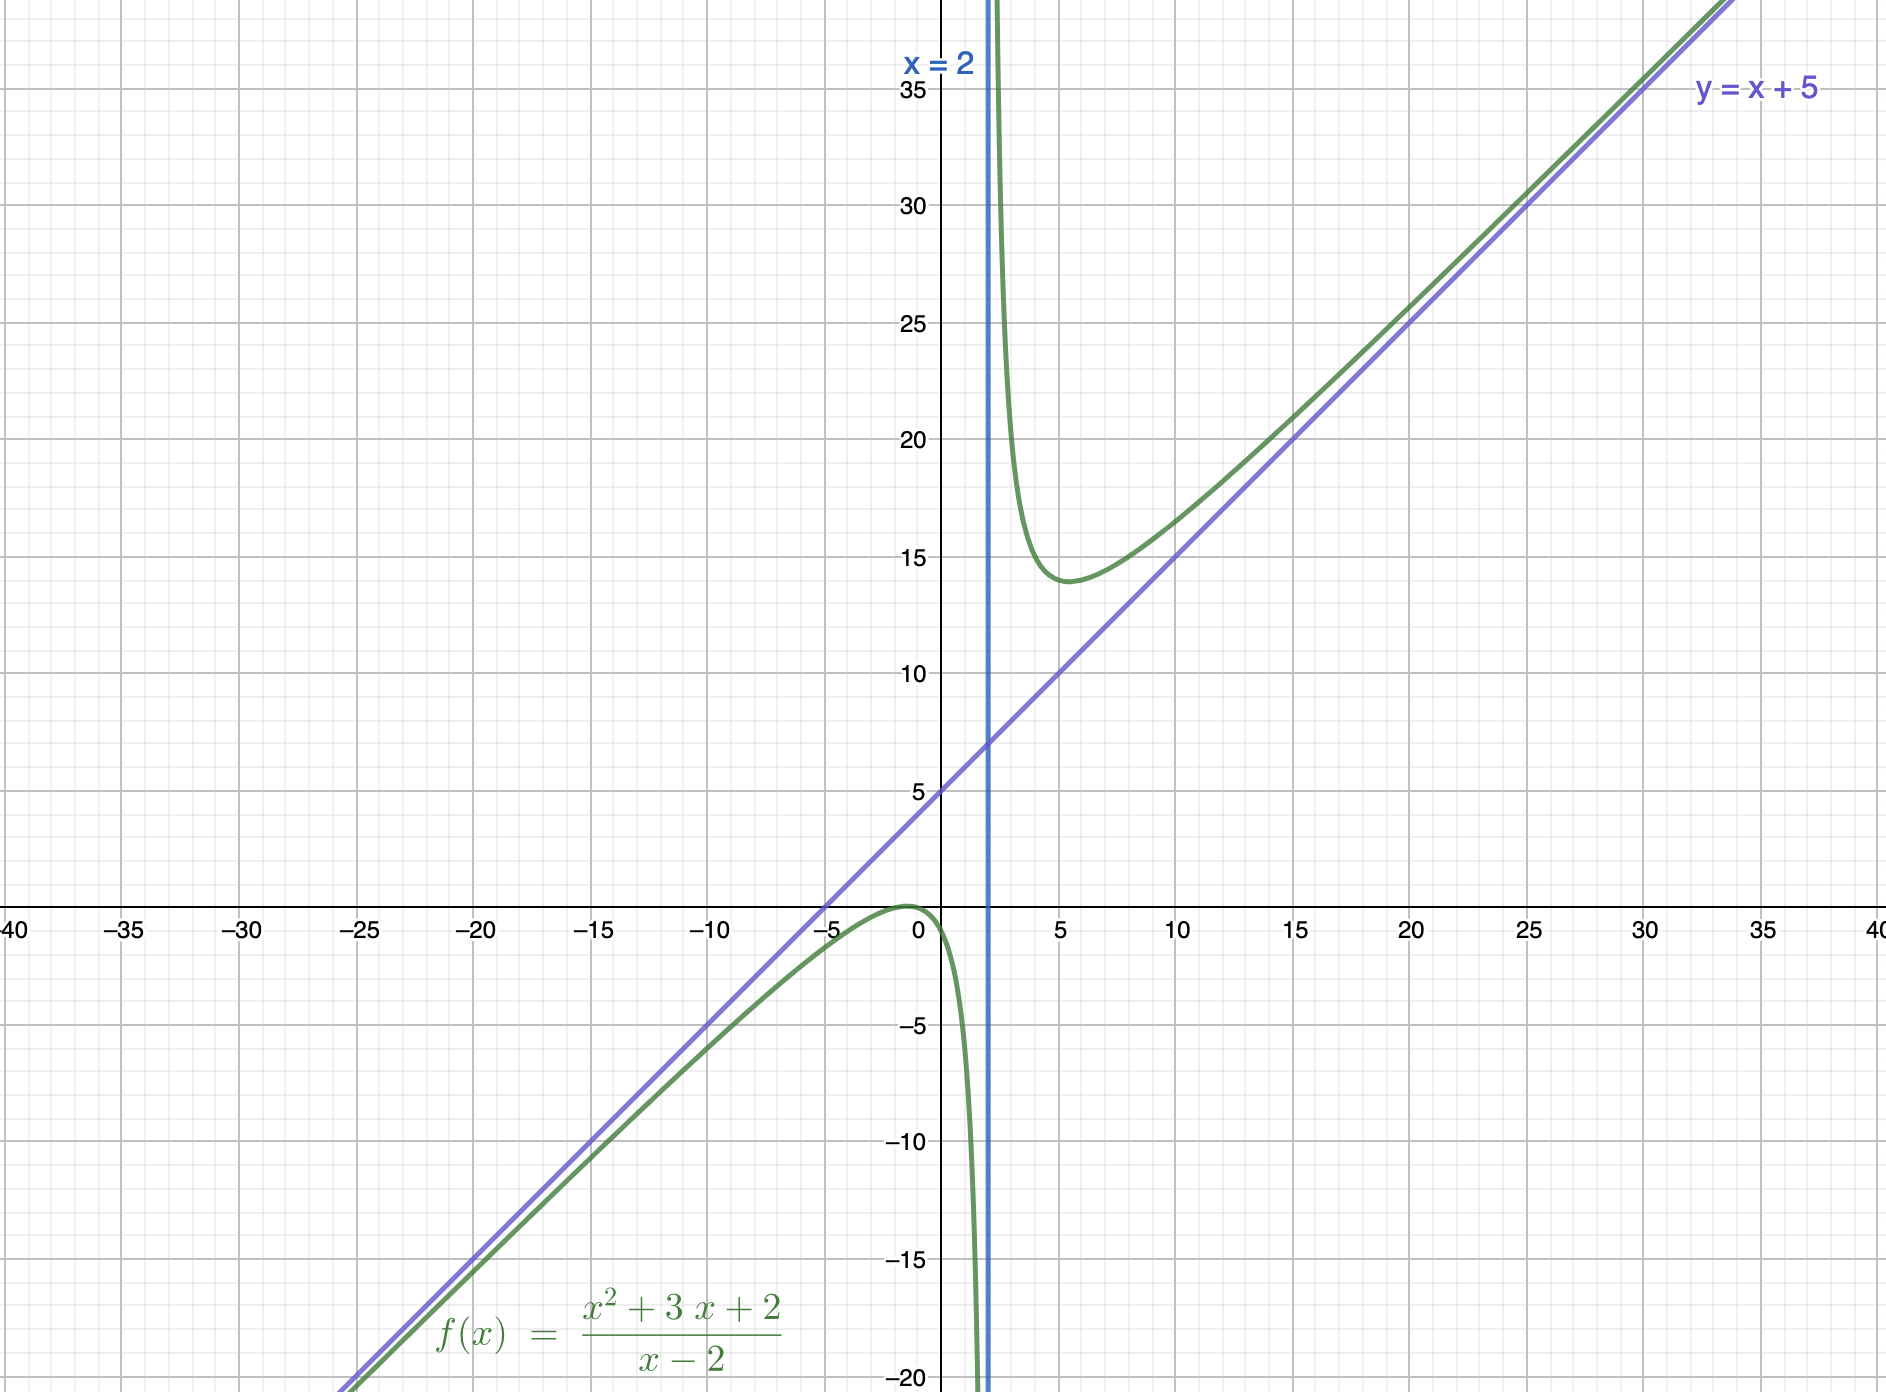
\includegraphics[width=0.8\textwidth]{Fig.2.8.jpg}
            \end{figure}
        \end{example}
        \begin{example}{2.4.6}{}
            \textbf{Draw the diagram of $\displaystyle y=\frac{x^2-x-2}{x-1}$.}\\
            \noindent\rule[0.1pt]{\textwidth}{1pt}
            Intercept: $\displaystyle\left(0,2\right),\ \left(2,0\right),\ \left(-1,0\right)$\\
            V.A.: $x=1$\\
            O.A.: $y=x$ (Use long division)
            \begin{figure}[H]
                \centering
                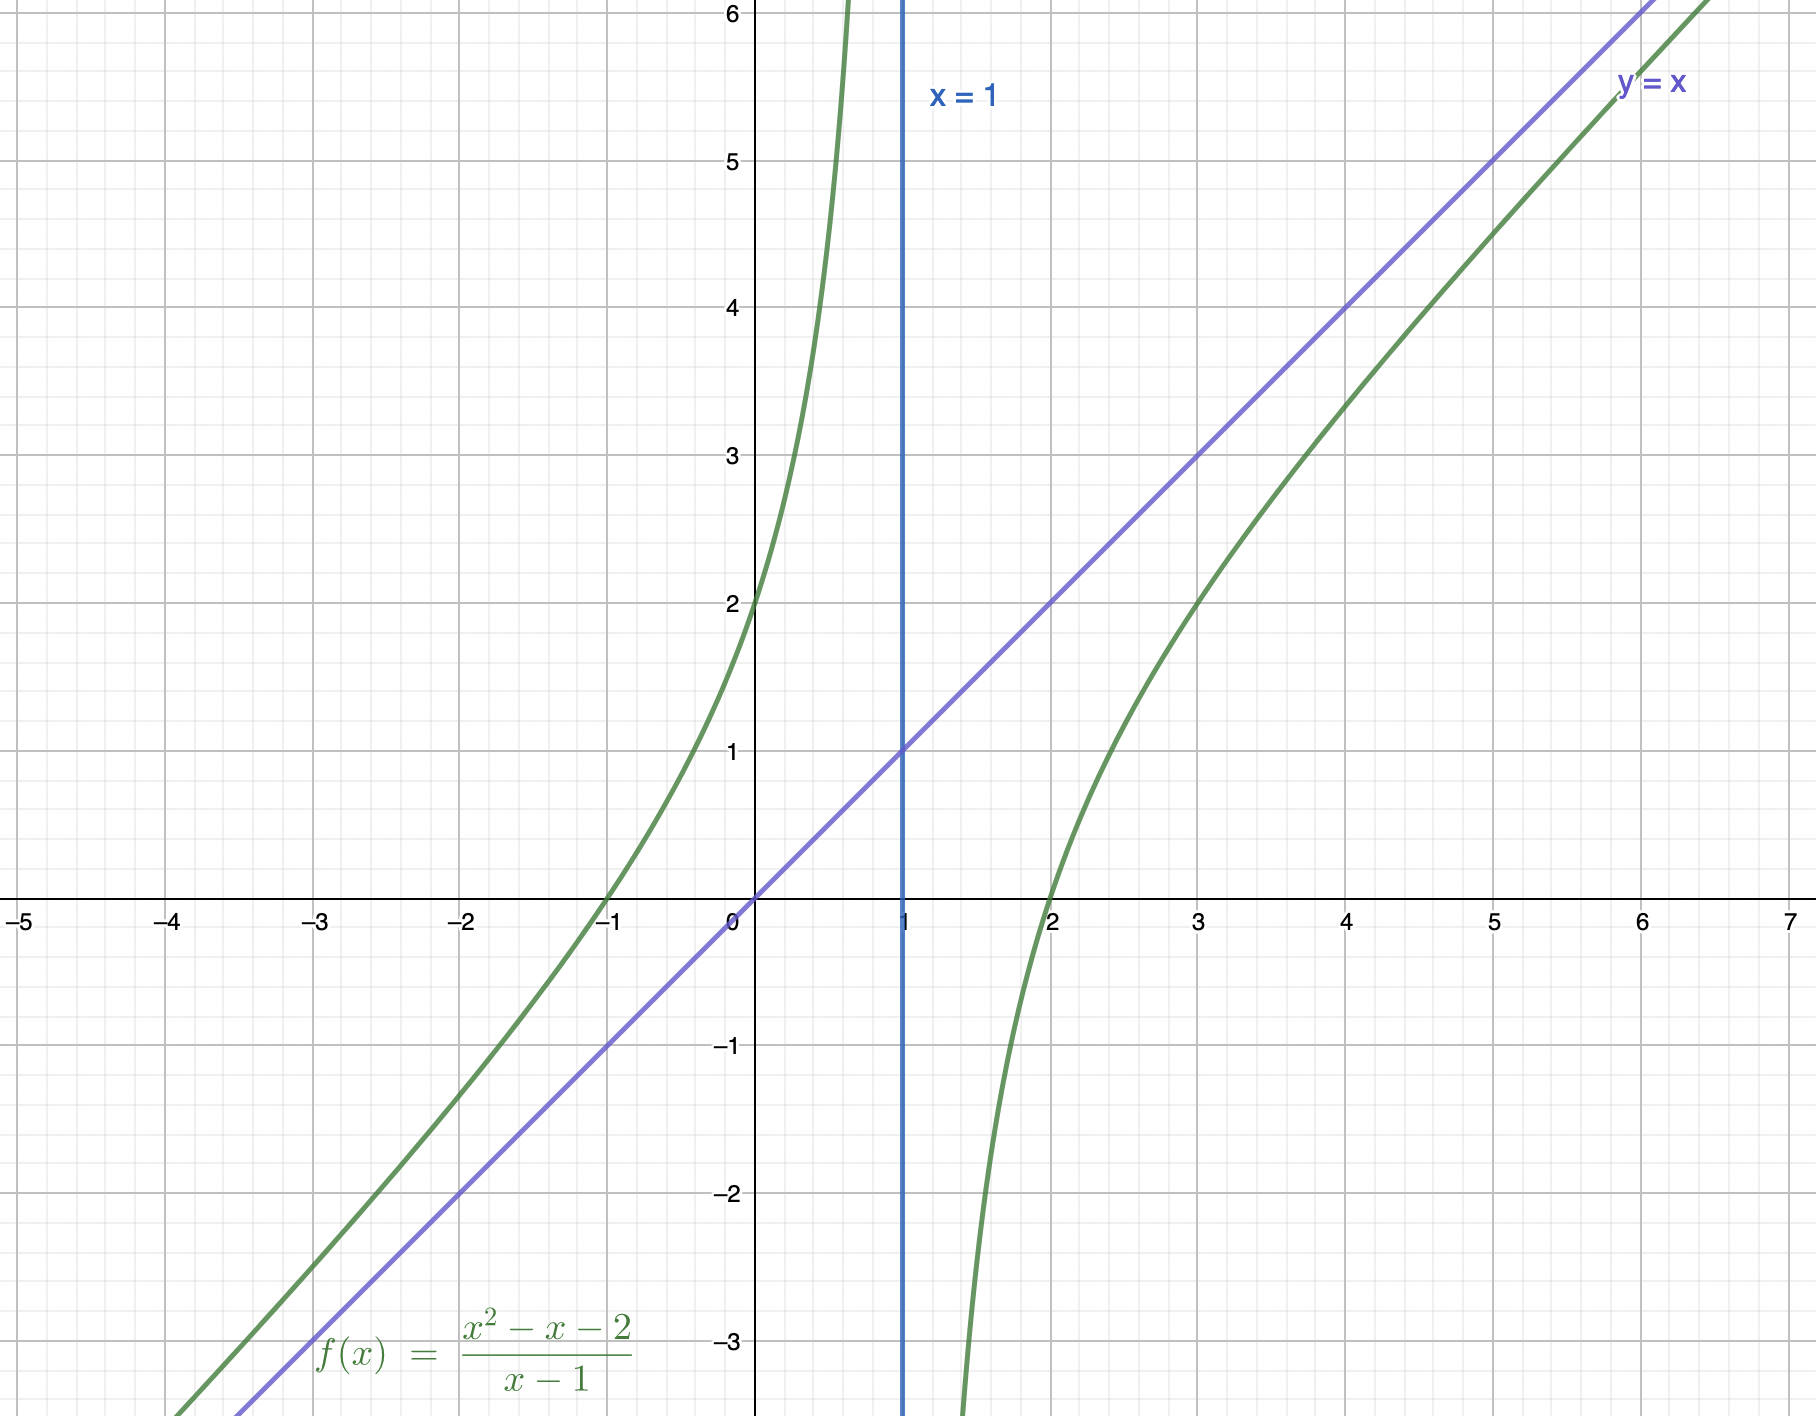
\includegraphics[width=0.8\textwidth]{Fig.2.9.jpg}
            \end{figure}
        \end{example}
    \end{itemize}
    \item When the function has asymptotes: 
    \begin{itemize}
        \item Denominator$=0$;
        \item $\log_a{0}$ (argument of a logarithm is 0)
    \end{itemize}
\end{enumerate}

\section{Transformation of Functions}
\begin{enumerate}
    \item \textbf{\color{red}{Translation}}: 
    \begin{itemize}
        \item $f(x+n)$ means translate $f(x)$ $n$ units to the left. 
        \item $f(x-n)$ means translate $f(x)$ $n$ units to the right. 
        \item $f(x)+n$ means translate $f(x)$ $n$ units upwards.
        \item $f(x)-n$ means translate $f(x)$ $n$ units downwards.
    \end{itemize}
    \item Use translation vector to represent translation: \\
    A vector ${\color{red}{\begin{pmatrix}a\\b\end{pmatrix}}}$ means $a$ units in the horizontal axis and $b$ units in the vertical axis. 
    \begin{example}{2.5.1}{}
        A translation vector $\begin{pmatrix}-2\\3\end{pmatrix}$ means $f(x+2)+3$, 2 units to the left and 3 units upwards. 
    \end{example}
    \item \textbf{\color{red}{Reflections}}: 
    \begin{itemize}
        \item $f(-x)$ reflects in the {\color{red}{$y$-axis}}. 
        \item $-f(x)$ reflects in the {\color{red}{$x$-axis}}. 
        \item $f^{-1}(x)$ reflects in the {\color{red}{$y=x$}}.
        \item $-f(-x)$ reflects in the {\color{red}{origin}}.  
    \end{itemize}
    \item \textbf{\color{red}{Stretches}}: 
    \begin{itemize}
        \item $f(qx)$ is a horizontal stretch of a scale factor of $\displaystyle\frac{1}{q}$.
        \item $pf(x)$ is a vertical stretch of a scale factor of $p$.
    \end{itemize}
    \item When a graph is transforming, the points shift but the connection remains. 
    \item Sequence of transformation: 
    \begin{itemize}
        \item Do the horizontal translation before the horizontal stretch.
        \item The vertical translation is always after the vertical stretch.
        \item Vertical stretch $\rightarrow$ Reflection $\rightarrow$ Horizontal translation $\rightarrow$ Horizontal stretch $\rightarrow$ Vertical translation
    \end{itemize}
    \item \textbf{\color{red}{Modulus Function}}
    \begin{itemize}
        \item ${\color{red}{\left|f(x)\right|}}$: Fold everything below $x$-axis above $x$-axis. 
        \begin{example}{2.5.2}{}
        \begin{figure}[H]
            \centering
            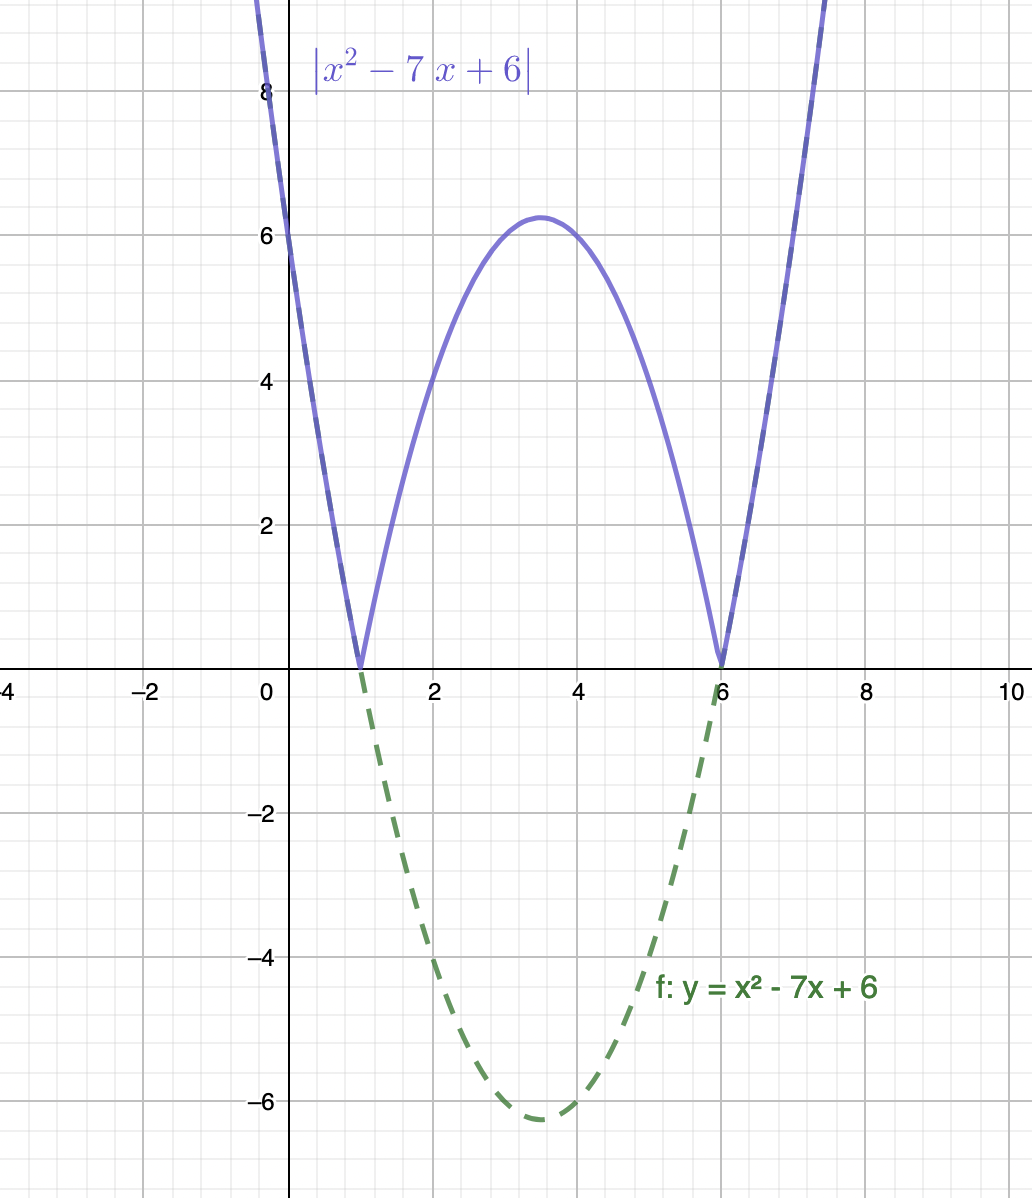
\includegraphics[width=0.48\textwidth]{Fig.2.10.jpg}
        \end{figure}
        \end{example}
        \item ${\color{red}{f(\left|x\right|)}}$: Reflect everthing on the right of $y$-axis to the left. 
        {\color{green}{Since $|x|$ must be positive, $|x|=|-x|\ \Rightarrow\ f(-x)=f(x)$, which is an even function.}}
        \begin{example}{2.5.3}{}
            \begin{figure}[H]
                \centering
                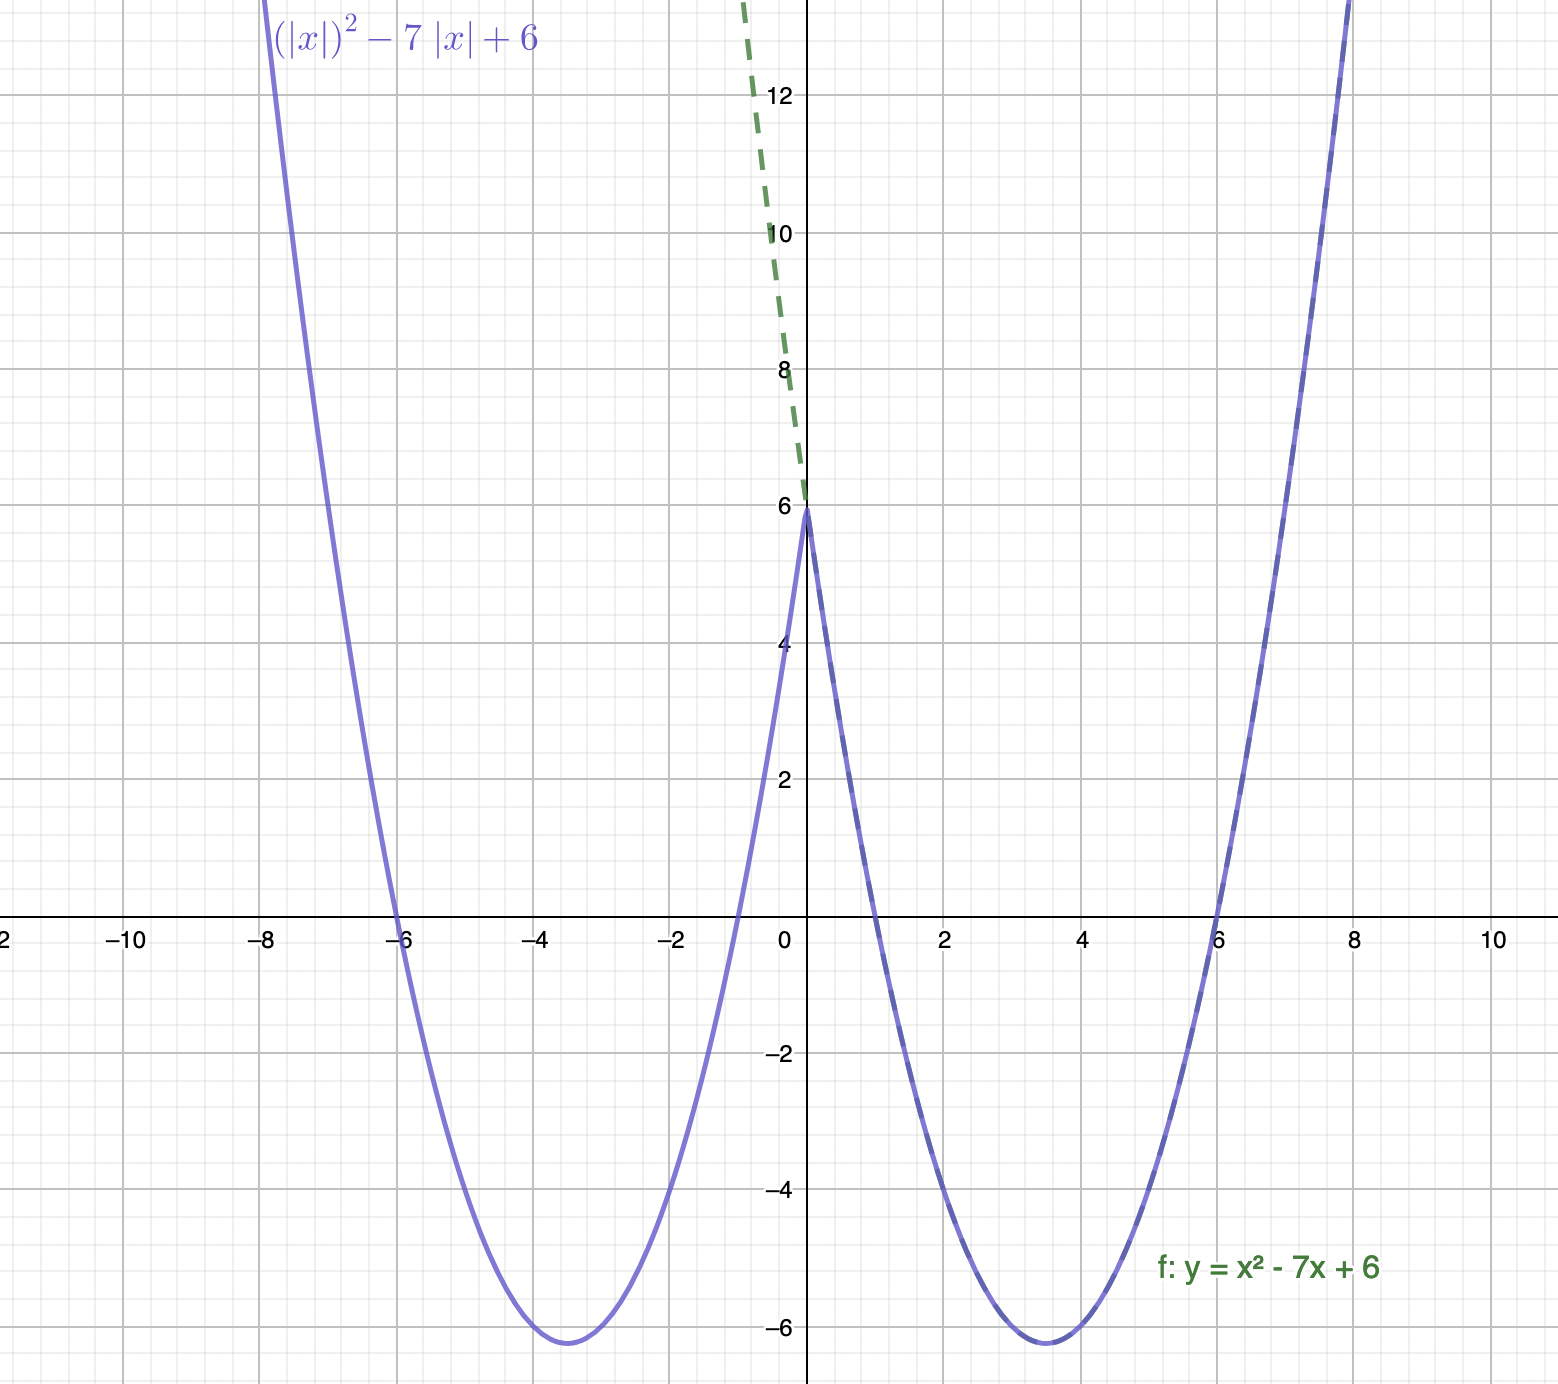
\includegraphics[width=0.6\textwidth]{Fig.2.11.jpg}
            \end{figure}
            \end{example}
    \end{itemize}
    \item \textbf{\color{red}{Reciprocal of $f(x)$}}
    \begin{itemize}
        \item Table of Summary: 
        \begin{center}
        \begin{tabular}{c|c}
            $f(x)$&$g(x)=\frac{1}{x}$\\\hline
            $f(a)=0$&Line $x=a$ is vertical asymptote\\\hline
            Line $x=a$ is vertical asymptote&$g(a)=0$\\\hline
            $f(x)\to\infty$&$g(x)\to 0$\\\hline
            $f(x)\to 0$&$g(x)\to\infty$\\\hline
            Line $y=b$ is horizontal asymptote&Line $y=\frac{1}{b}$ is horizontal asymptote\\\hline
            $f(x)=a$&$g(x)=\frac{1}{a}$
        \end{tabular}
        \end{center}
        \item When $f(x)$ increases, $g(x)$ decreases. 
    \end{itemize}
\end{enumerate}

\section{Exponential and Logarithmic Functions}
\begin{enumerate}
    \item Exponential functions: 
    \begin{itemize}
        \item $f(x)=a^x,\ a>1$ (increasing) and $0<a<1$ (decreasing). 
        \item $f(x)=a^x$ and $g(x)=\displaystyle\left(\frac{1}{a}\right)^x$ are symmetric to the $y$-axis. 
        \begin{proof}{2.6.1}{}
            $$g(x)=\left(\frac{1}{a}\right)^x=(a^-1)^x=a^{-x}=f(-x).$$
        \end{proof}
        \item Domain: $x\in\R$, Range: $y>0$
        \item Common point: $(0, 1)$; common H.A.: $y=0$
        \item Graph: 
        \begin{figure}[H]
            \centering
            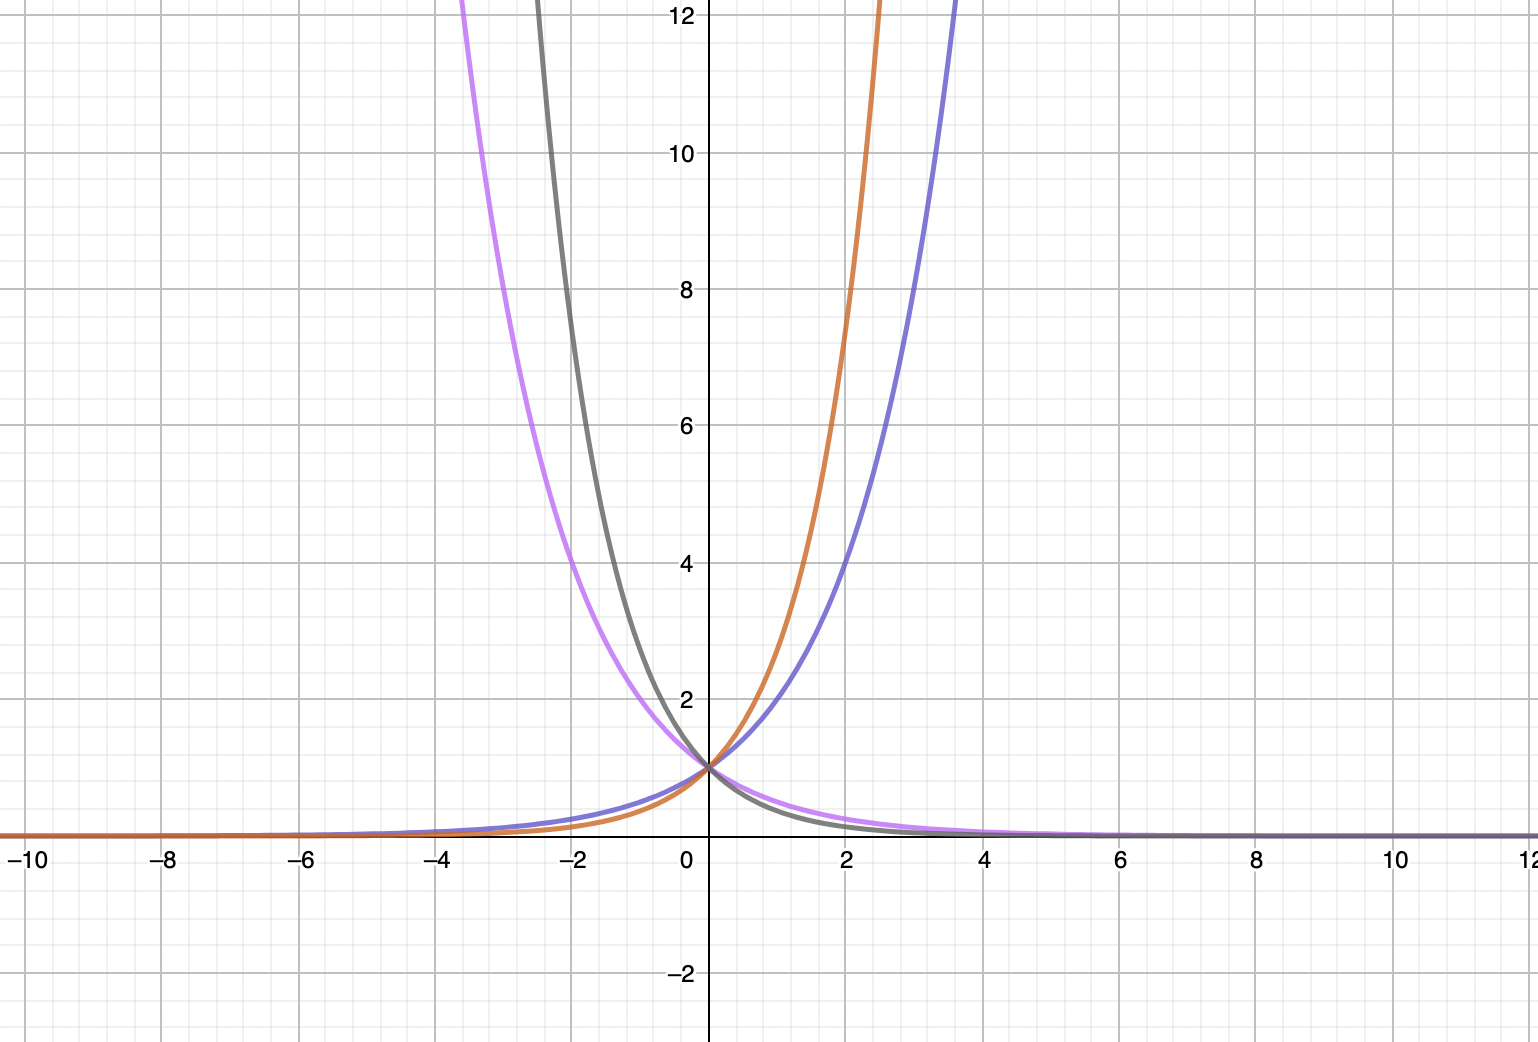
\includegraphics[width=0.48\textwidth]{Fig.2.12.jpg}
        \end{figure}
    \end{itemize}
    \item Logarithmic functions: 
    \begin{itemize}
        \item $f(x)=\log_a{x}=g^{-1}(x), g(x)=a^x$.
        \item Common point: $(1,0)$; common V.A.: $x=0$.
        \item $f(x)=\log_a{x}$ and $g(x)=\log_{\frac{1}{a}}{x}$ are symmetric to the $x$-axis.
        \begin{proof}{2.6.2}{}
            $$\log_{\frac{1}{a}}{x}=\frac{\log_a{x}}{\log_\frac{1}{a}a}=\frac{\log_ax}{-1}=-\log_ax,$$
            $$\therefore g(x)=\log_\frac{1}{a}x=-\log_ax=-f(x).$$
        \end{proof}
        \item When $a>1$, increasing function; when $0<a<1$, decreasing function. 
        \item Domain: $x>0$, Range: $y\in\R$
        \item Graph: 
        \begin{figure}[H]
            \centering
            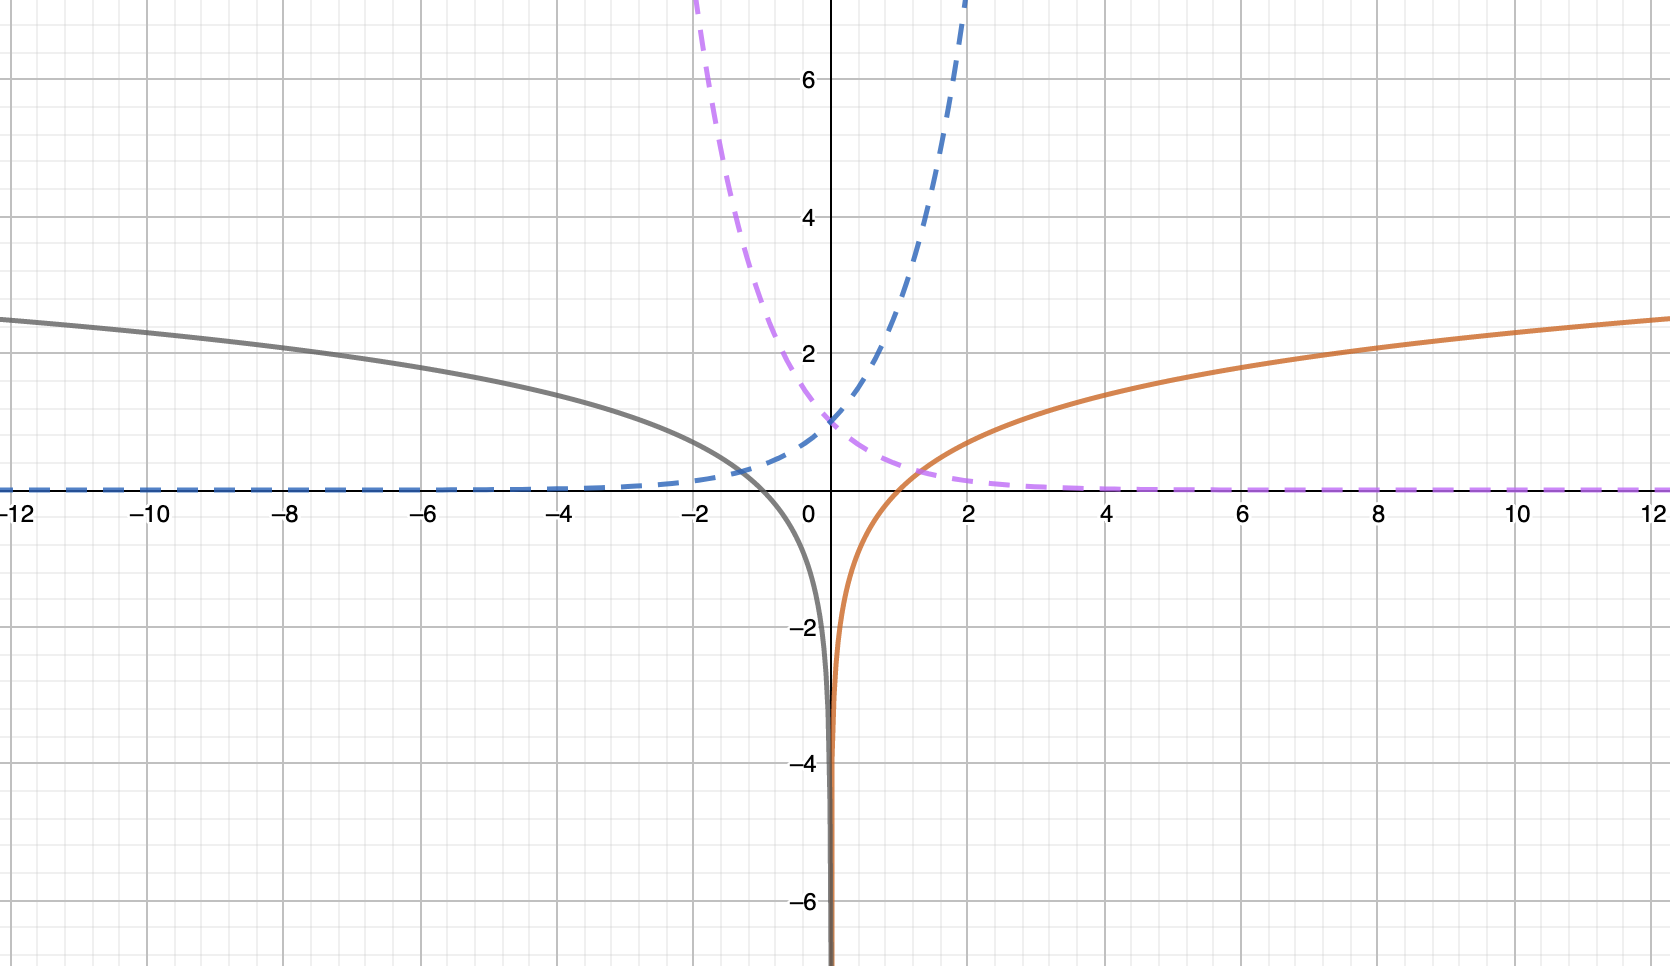
\includegraphics[width=0.7\textwidth]{Fig.2.13.jpg}
        \end{figure}
    \end{itemize}
    \item Solving logarithmic equations.
    \item Solving exponential equations: take logarithm on both sides.
\end{enumerate}

\end{document}